%\RequirePackage[l2tabu, orthodox]{nag}
\RequirePackage{currfile}
\documentclass[12pt]{beamer}
\graphicspath{{Imagenes/}{../Imagenes/}}
\usepackage[utf8]{inputenc}
\usepackage[spanish]{babel}
\usepackage{standalone}
\usepackage{color}
\usepackage[binary-units=true]{siunitx}
\usepackage{hyperref}
\hypersetup{
  colorlinks=true,
  linkcolor=blue,          % color of internal links (change box color with linkbordercolor)
  citecolor=green,        % color of links to bibliography
  filecolor=magenta,      % color of file links
  urlcolor=cyan,           % color of external links
  linkbordercolor={0 0 1}
}
\usepackage{xcolor, soul}
\usepackage{etoolbox}
\usepackage{amsmath}
\usepackage{amsthm}
\usepackage{physics}
\usepackage{multicol}
\usepackage{graphicx}
\usepackage{bookmark}
\usepackage{longtable}
\usepackage{graphicx}
\usepackage{tikz}
\usepackage[siunitx, RPvoltages]{circuitikz}
\usetikzlibrary{mindmap}
\usetikzlibrary{arrows, patterns, shapes, decorations.markings, decorations.pathmorphing}
\usetikzlibrary{matrix,positioning}
\tikzstyle{every picture}+=[remember picture,baseline]
\usepackage[autostyle,spanish=mexican]{csquotes}
\usepackage{pifont}
\usepackage[font=footnotesize,textfont=it]{caption}
\usepackage{tabulary}
\usepackage{booktabs}
\usepackage[outdir=./]{epstopdf}
%\usepackage{epstopdf}
\usepackage{media9}
\usepackage{multimedia}
\usepackage{bigints}
%\usepackage{enumitem}
\usepackage[os=win]{menukeys}
\usepackage{pifont}
\usepackage{pbox}
\usepackage{alltt}
\usepackage{verbatim}
\usepackage{colortbl}
\usepackage{tcolorbox}
\usepackage{fancyvrb}
\usepackage[sfdefault]{roboto}  %% Option 'sfdefault' only if the base font of the document is to be sans serif
%\usepackage[T1]{fontenc}
\setcounter{secnumdepth}{3}
\setcounter{tocdepth}{3}
\DeclareGraphicsExtensions{.pdf,.png,.jpg}
\renewcommand {\arraystretch}{1.5}
\definecolor{ao}{rgb}{0.0, 0.5, 0.0}
\definecolor{aquamarine}{rgb}{0.5, 1.0, 0.83}
\definecolor{kellygreen}{rgb}{0.3, 0.73, 0.09}
\definecolor{bisque}{rgb}{1.0, 0.89, 0.77}
\definecolor{amber}{rgb}{1.0, 0.75, 0.0}
\definecolor{armygreen}{rgb}{0.29, 0.33, 0.13}
\definecolor{alizarin}{rgb}{0.82, 0.1, 0.26}
\definecolor{cadetblue}{rgb}{0.37, 0.62, 0.63}
\newcommand*{\TitleParbox}[1]{\parbox[c]{6cm}{\raggedright #1}}%
\newcommand{\python}{\texttt{python}}
\newcommand{\textoazul}[1]{\textcolor{blue}{#1}}
\newcommand{\azulfuerte}[1]{\textcolor{blue}{\textbf{#1}}}
\newcommand{\funcionazul}[1]{\textcolor{blue}{\textbf{\texttt{#1}}}}
%\normalfont
\usepackage{ccfonts}% http://ctan.org/pkg/{ccfonts}
\usepackage[T1]{fontenc}% http://ctan.or/pkg/fontenc
\renewcommand{\rmdefault}{cmr}% cmr = Computer Modern Roman
\usefonttheme[onlymath]{serif}
\linespread{1.3}
\newcounter{saveenumi}
\newcommand{\seti}{\setcounter{saveenumi}{\value{enumi}}}
\newcommand{\conti}{\setcounter{enumi}{\value{saveenumi}}}
\newcommand{\tikzmark}[1]{\tikz[remember picture] \node[coordinate] (#1) {#1};}

\usepackage{scalerel}[2016-12-29]
\def\stretchint#1{\vcenter{\hbox{\stretchto[440]{\displaystyle\int}{#1}}}}
\def\scaleint#1{\vcenter{\hbox{\scaleto[3ex]{\displaystyle\int}{#1}}}}
\def\bs{\mkern-12mu}

\newtheorem{teo}{}[section]
\usepackage{blkarray}

%reduce el tamaño de letra de la etiqueta equations
\makeatletter
\def\maketag@@@#1{\hbox{\m@th\normalfont\small#1}}
\makeatother

%se usa para la x en itemize
\newcommand{\xmark}{\text{\ding{55}}}

%\AtBeginDocument{\setlength{\tymin}{1em}}


\definecolor{myblue}{rgb}{.8, .8, 1}

\usepackage{empheq}

\newlength\mytemplen
\newsavebox\mytempbox

\makeatletter
\newcommand\mybluebox{%
    \@ifnextchar[%]
       {\@mybluebox}%
       {\@mybluebox[0pt]}}

\def\@mybluebox[#1]{%
    \@ifnextchar[%]
       {\@@mybluebox[#1]}%
       {\@@mybluebox[#1][0pt]}}

\def\@@mybluebox[#1][#2]#3{
    \sbox\mytempbox{#3}%
    \mytemplen\ht\mytempbox
    \advance\mytemplen #1\relax
    \ht\mytempbox\mytemplen
    \mytemplen\dp\mytempbox
    \advance\mytemplen #2\relax
    \dp\mytempbox\mytemplen
    \colorbox{myblue}{\hspace{1em}\usebox{\mytempbox}\hspace{1em}}}

\makeatother



%Se usa la plantilla Warsaw modificada con spruce
\mode<presentation>
{
  \usetheme{Warsaw}
  \setbeamertemplate{headline}{}
  \useoutertheme{default}
  %\usecolortheme{beaver}
  \setbeamercovered{invisible}
}
%\AtBeginSection[]
%{
%\begin{frame}<beamer>{Contenido}
%\normalfont\mdseries
%\tableofcontents[currentsection]
%\end{frame}
%}

\setbeamertemplate{section in toc}[sections numbered]
\setbeamertemplate{subsection in toc}[subsections numbered]
\setbeamertemplate{subsection in toc}{\leavevmode\leftskip=3.2em\rlap{\hskip-2em\inserttocsectionnumber.\inserttocsubsectionnumber}\inserttocsubsection\par}
\setbeamercolor{section in toc}{fg=blue}
\setbeamercolor{subsection in toc}{fg=blue}
\setbeamertemplate{navigation symbols}{}
\setbeamercolor{frametitle}{fg=yellow,bg=blue!70!white}
\setbeamercolor{section in head/foot}{bg=gray!30,fg=red}
%\setbeamercolor{section in head}{bg=green,fg=red}
\setbeamercolor{subsection in head/foot}{bg=gray!30,fg=black}
\setbeamercolor{author in head/foot}{bg=gray!30}
\setbeamercolor{date in head/foot}{fg=blue}

%\mode<presentation>
%{
%  \usetheme{Warsaw}
%  \setbeamertemplate{headline}{}
%  %\useoutertheme{infolines}
%  \useoutertheme{default}
%  \setbeamercovered{invisible}
%  % or whatever (possibly just delete it)
%}

\usepackage{courier}
\usepackage{listingsutf8}
\usepackage{listings}
\usepackage{xcolor}
\usepackage{textcomp}
\usepackage{color}
\definecolor{deepblue}{rgb}{0,0,0.5}
\definecolor{brown}{rgb}{0.59, 0.29, 0.0}
\definecolor{OliveGreen}{rgb}{0,0.25,0}
% \usepackage{minted}

\DeclareCaptionFont{white}{\color{white}}
\DeclareCaptionFormat{listing}{\colorbox{gray}{\parbox{0.98\textwidth}{#1#2#3}}}
\captionsetup[lstlisting]{format=listing,labelfont=white,textfont=white}
\renewcommand{\lstlistingname}{Código}


\definecolor{Code}{rgb}{0,0,0}
\definecolor{Keywords}{rgb}{255,0,0}
\definecolor{Strings}{rgb}{255,0,255}
\definecolor{Comments}{rgb}{0,0,255}
\definecolor{Numbers}{rgb}{255,128,0}

\makeatletter

\newif\iffirstchar\firstchartrue
\newif\ifstartedbyadigit
\newif\ifprecededbyequalsign

\newcommand\processletter
{%
  \ifnum\lst@mode=\lst@Pmode%
    \iffirstchar%
        \global\startedbyadigitfalse%
      \fi
      \global\firstcharfalse%
    \fi
}

\newcommand\processdigit
{%
  \ifnum\lst@mode=\lst@Pmode%
      \iffirstchar%
        \global\startedbyadigittrue%
      \fi
      \global\firstcharfalse%
  \fi
}

\lst@AddToHook{OutputOther}%
{%
  \lst@IfLastOtherOneOf{=}
    {\global\precededbyequalsigntrue}
    {}%
}

\lst@AddToHook{Output}%
{%
  \ifprecededbyequalsign%
      \ifstartedbyadigit%
        \def\lst@thestyle{\color{orange}}%
      \fi
    \fi
  \global\firstchartrue%
  \global\startedbyadigitfalse%
  \global\precededbyequalsignfalse%
}

\lstset{ 
language=Python,                % choose the language of the code
basicstyle=\footnotesize\ttfamily,       % the size of the fonts that are used for the code
numbers=left,                   % where to put the line-numbers
numberstyle=\scriptsize,      % the size of the fonts that are used for the line-numbers
stepnumber=1,                   % the step between two line-numbers. If it is 1 each line will be numbered
numbersep=5pt,                  % how far the line-numbers are from the code
backgroundcolor=\color{white},  % choose the background color. You must add \usepackage{color}
showspaces=false,               % show spaces adding particular underscores
showstringspaces=false,         % underline spaces within strings
showtabs=false,                 % show tabs within strings adding particular underscores
frame=single,   		% adds a frame around the code
tabsize=2,  		% sets default tabsize to 2 spaces
captionpos=t,   		% sets the caption-position to bottom
breaklines=true,    	% sets automatic line breaking
breakatwhitespace=false,    % sets if automatic breaks should only happen at whitespace
escapeinside={\#},  % if you want to add a comment within your code
stringstyle =\color{OliveGreen},
%otherkeywords={{as}},             % Add keywords here
keywordstyle = \color{blue},
commentstyle = \color{black},
identifierstyle = \color{black},
literate=%
         {á}{{\'a}}1
         {é}{{\'e}}1
         {í}{{\'i}}1
         {ó}{{\'o}}1
         {ú}{{\'u}}1
%
%keywordstyle=\ttb\color{deepblue}
%fancyvrb = true,
}

\lstdefinestyle{FormattedNumber}{%
    literate={0}{{\textcolor{red}{0}}}{1}%
             {1}{{\textcolor{red}{1}}}{1}%
             {2}{{\textcolor{red}{2}}}{1}%
             {3}{{\textcolor{red}{3}}}{1}%
             {4}{{\textcolor{red}{4}}}{1}%
             {5}{{\textcolor{red}{5}}}{1}%
             {6}{{\textcolor{red}{6}}}{1}%
             {7}{{\textcolor{red}{7}}}{1}%
             {8}{{\textcolor{red}{8}}}{1}%
             {9}{{\textcolor{red}{9}}}{1}%
             {.0}{{\textcolor{red}{.0}}}{2}% Following is to ensure that only periods
             {.1}{{\textcolor{red}{.1}}}{2}% followed by a digit are changed.
             {.2}{{\textcolor{red}{.2}}}{2}%
             {.3}{{\textcolor{red}{.3}}}{2}%
             {.4}{{\textcolor{red}{.4}}}{2}%
             {.5}{{\textcolor{red}{.5}}}{2}%
             {.6}{{\textcolor{red}{.6}}}{2}%
             {.7}{{\textcolor{red}{.7}}}{2}%
             {.8}{{\textcolor{red}{.8}}}{2}%
             {.9}{{\textcolor{red}{.9}}}{2}%
             {\ }{{ }}{1}% handle the space
         ,%
          %mathescape=true
          escapeinside={__}
          }



\makeatletter
\setbeamertemplate{footline}
{
  \leavevmode%
  \hbox{%
  \begin{beamercolorbox}[wd=.333333\paperwidth,ht=2.25ex,dp=1ex,center]{author in head/foot}%
    \usebeamerfont{author in head/foot} \insertsection
  \end{beamercolorbox}}%
  \begin{beamercolorbox}[wd=.333333\paperwidth,ht=2.25ex,dp=1ex,center]{title in head/foot}%
    \usebeamerfont{title in head/foot} \insertsubsection
  \end{beamercolorbox}%
  \begin{beamercolorbox}[wd=.333333\paperwidth,ht=2.25ex,dp=1ex,right]{date in head/foot}%
    \usebeamerfont{date in head/foot} \textcolor{white}{\insertshortdate{}} \hspace*{2em}
    \textcolor{white}{\insertframenumber{} / \inserttotalframenumber}\hspace*{2ex} 
  \end{beamercolorbox}}%
  \vskip0pt%
\makeatother
\title{\large{Tema 1 - Escalas, condición y estabilidad}}
\subtitle{Curso de Física Computacional}
\author[]{M. en C. Gustavo Contreras Mayén}
\date{\today}
\institute{Facultad de Ciencias - UNAM}
\titlegraphic{
\includegraphics[width=2cm]{Imagenes/escudo-facultad-ciencias}\hspace*{4.75cm}~%
   
\includegraphics[width=2cm]{Imagenes/escudo-unam}
}
\begin{document}
\maketitle
\section*{Contenido}
\frame[allowframebreaks]{\tableofcontents[currentsection, hideallsubsections]}
\fontsize{14}{14}\selectfont
\spanishdecimal{.}
\section{Precisión de la máquina}
\frame{\tableofcontents[currentsection, hideothersubsections]}
\subsection{Precisión en punto flotante}
\begin{frame}
\frametitle{Precisión de la máquina}
Una preocupación importante en el cálculo computacional para la representación en punto flotante que se utliza para almacenar números es que se cuenta con una precisión limitada.
\end{frame}
\begin{frame}
\frametitle{Precisión de la máquina}
Como hemos visto, para una máquina de $32$ bits, los números de precisión simple son buenos para $6-7$ decimales, mientras que los de precisión doble son buenos para $15-16$ lugares.
\\
\bigskip
\pause
Para ver cómo la precisión limitada afecta a los cálculos, consideremos la suma en la computadora de dos palabras de precisión simple:
\\
\bigskip
\pause
\[ 7 + 1.0 \times 10^{-7} \]
\end{frame}
\begin{frame}
\frametitle{Representación de los valores}
La comptuadora extrae estos números de la memoria y los almacena en cadenas de bits
\fontsize{12}{12}\selectfont
\begin{eqnarray*}
7 &=& 0 \; 10000010 \; 1110 \: 0000 \: 0000 \: 0000 \: 0000 \: 000 \label{eq:ecuacion_01_10} \\
10^{-7} &=& 0 \; 01100000 \; 1101 \: 0110 \: 1011 \: 1111 \: 1001 \: 010 \label{eq:ecuacion_01_11}
\end{eqnarray*}
\end{frame}
\begin{frame}
\frametitle{Suma de los dos números}
Debido a que los exponentes son diferentes, no es correcto sumar las mantisas, y así el exponente del número más pequeño se hace más grande mientras que disminuye progresivamente la mantisa desplazando bits a la derecha (insertando ceros) hasta que ambos números tengan el mismo exponente.
\end{frame}
\begin{frame}
\fontsize{12}{12}\selectfont
\begin{eqnarray*}
10^{-7} &=& 0 \; 01100000 \; 1101 \: 0110 \: 1011 \: 1111 \: 1001 \: 010 \\ \pause
&=& 0 \; 01100001 \; 0110 \: 1011 \: 0101 \: 1111 \: 1100 \: 101 \: (0) \\ \pause
&=& 0 \; 01100010 \; 0011 \: 0101 \: 1010 \: 1111 \: 1110 \: 010 \: (10) \\ \pause
&\ldots& \\ \pause
&=& 0 \; 10000010 \; 0000 \: 0000 \: 0000 \: 0000 \: 00000 \: 000 \: (0001101 \ldots 0) \\
&\rightarrow& 7 +1.0 \times 10^{-7} = 7
\label{eq:ecuacion_01_12}
\end{eqnarray*}
\end{frame}
\begin{frame}
\frametitle{Dígitos significativos}
Debido a que no hay espacio para almacenar los últimos dígitos, éstos se pierden, y después de todo este largo proceso, la suma sólo devuelve $7$ como respuesta (tenemos un error de truncamiento)
\\
\bigskip
\pause
En otras palabras, debido a que un equipo de $32$ bits almacena sólo $6$ o $7$ decimales, ignora efectivamente cualquier cambio más allá del sexto decimal.    
\end{frame}
\subsection{Definición de la precisión de la máquina}
\begin{frame}
\frametitle{Precisión de la máquina}
La pérdida de precisión anterior se categoriza definiendo la precisión de la máquina $\epsilon_{m}$ como el máximo número positivo que en la computadora, se puede sumar al número almacenado como $1$ sin cambiarlo:    
\begin{equation}
1_{c} + \epsilon_{m} = 1_{c}
\label{eq:ecuacion_01_14}
\end{equation}
\end{frame}
\begin{frame}
Por consiguiente, un número arbitrario $x$ puede considerarse relacionado con su representación en punto flotante $x_{c}$ por
\[ x_{c} = x(1 \pm \epsilon) \hspace{1cm} \vert \epsilon \vert \leq \epsilon_{m} \]
donde no se conoce el valor real de $\epsilon$.
\end{frame}
\begin{frame}
En otras palabras, con excepción de las potencias de $2$ que están representadas exactamente, debemos suponer que todos los números de precisión simple contienen un error en el sexto decimal y que todos los dobles tienen un error en el decimoquinto lugar.
 \end{frame}
 \begin{frame}
Y como siempre ocurre con los errores, debemos suponer que no sabemos cuál es el error, porque si lo supiéramos: \textoazul{¡entonces lo eliminaríamos!}
\\
\bigskip
En consecuencia, los argumentos que planteamos con respecto a los errores son siempre aproximados, y eso es lo mejor que podemos hacer.
\end{frame}
\subsection{Calculando la precisión de la máquina}
\begin{frame}
\frametitle{El epsilón de la máquina}
\begin{figure}
\centering
\includestandalone[scale=0.7]{Figuras/epsilonmaquina}
\end{figure}
\end{frame}
\begin{frame}
\frametitle{Calculando el epsilón de la máquina}
Una tarea inicial que debemos de atender, es el cálculo de la precisión de la máquina, a la que llamaremos  \azulfuerte{epsilón de la máquina}.
\\
\bigskip
\pause
Veamos cómo calcular con \python ese valor:
\end{frame}
\begin{frame}
\frametitle{Punto de partida}
\fontsize{10}{10}\selectfont
\begin{figure}
\centering
\includestandalone{Figuras/epsilonmaquina_02}
\end{figure}
\end{frame}
\begin{frame}[fragile]
\frametitle{Calculemos el epsilón con \python}
\begin{lstlisting}[style= FormattedNumber, basicstyle=\linespread{0.9}\ttfamily\normalsize, columns=fullflexible]
t = 1.0;

while 1 + t != 1:
    eps = t
    t = t/2

print ('el epsilon de la maquina es: ', eps)
\end{lstlisting}
\pause
En mi equipo obtengo el siguiente resultado:
\\
El cero de la maquina es:  $2.220446049250313e-16$
\end{frame}
% \begin{frame}
% \frametitle{Ejercicio más elaborado}
% Un problema clásico es la suma de los términos de una serie para evaluar una función.
% \\
% \bigskip
% Considera la serie infinita que representa la función $\sin \: x$:
% \[ \sin \: x = x - \dfrac{x^{3}}{3!} + \dfrac{x^{5}}{5!} + \dfrac{x^{7}}{7!} + \ldots \]
% \end{frame}
% \begin{frame}
% \frametitle{Propuesta de algoritmo}
% Nuestro problema es usar la serie para calcular valores de $\sin \: x$ para $x < 2 \pi$ y $x > 2 \pi$, con un error absoluto en cada caso, menor a $1$ parte en $10^{8}$.
% \pause
% Como la serie infinita es \emph{exacta} en el sentido matemático, no es una buena propuesta de algoritmo, ya que se necesita hacer un alto en algún momento.
% \end{frame}
% \begin{frame}\frametitle{Cambio a una serie finita}
% Un algoritmo para una suma finita sería:
% \begin{equation}
% \sin \: x \simeq \sum_{n = 1}^{N} \dfrac{(-1)^{n-1} \: x^{2n-1}}{(2n -1)!}
% \label{eq:ecuacion_01_15}
% \end{equation}
% \pause
% ¿Pero en qué momento detenemos la suma?
% \end{frame}
% \begin{frame}
% \frametitle{Lo que nos dice el algoritmo}
% No debemos de pensar que con el algoritmo anterior (\ref{eq:ecuacion_01_15}), nos dice que calculemos $(-1)^{n-1} \: x^{2n-1}$ para luego dividir por $(2n-1)!$. No es una buena idea!!
% \end{frame}
% \begin{frame}
% \frametitle{Como resolver la suma}
% Por una parte, tanto $(2n-1)!$ y $x^{2n-1}$ pueden ser operaciones extendidas y generar overflow.
% \\
% \bigskip
% Y por otra, el cálculo de potencias y factoriales demandan demasiado tiempo de cálculo, por lo que debemos de buscar una alternativa. 
% \end{frame}
% \begin{frame}
% \frametitle{Relacionando los términos}
% Nos conviene utilizar una expresión que evalúe un producto y que relacione el siguiente término de la serie con el anterior:
% \begin{align}
% \begin{aligned}
% \dfrac{(-1)^{n-1} \: x^{2n-1}}{(2n-1)!} &=& \dfrac{x^{2}}{(2n - 1)(2n - 2)} \dfrac{(-1)^{n-2} \: x^{2n - 3}}{(2n - 3)!} \\
% \rightarrow  n_{\text(esimo)} &=& \dfrac{x^{2}}{(2n - 1)(2n - 2)} \times n-1_{\text{esimo}}
% \end{aligned}
% \label{eq:ecuacion_01_16}
% \end{align}
% \end{frame}
% \begin{frame}
% \frametitle{Detener la suma}
% Si bien queremos asegurar una exactitud definida para el valor de $\sin \: x$, esto no es tan fácil de hacer.
% \\
% \bigskip
% \pause
% Lo que es fácil de hacer es suponer que el error en la suma es aproximadamente el último término sumado (esto no supone ningún error de redondeo)
% \end{frame}
% \begin{frame}
% \frametitle{Detener la suma}
% Para obtener un error absoluto de $1$ parte en $10^{-8}$, entonces detenemos el cálculo cuando
% \begin{equation}
% \left| \dfrac{n_{\text{esimo}}}{suma} \right| < 10^{-8}
% \label{eq:ecuacion_01_17}
% \end{equation}
%  Donde el n-ésimo es el último término que se guarda en la serie (\ref{eq:ecuacion_01_15}) y la suma, es la suma acumulada de todos los términos.
% \end{frame}
\section{Tipos de errores}
\frame{\tableofcontents[currentsection, hideothersubsections]}
\begin{frame}
\frametitle{Nuevos conceptos}
Una vez que se ha establecido la clasificación del error, definiremos los conceptos de:
\begin{itemize}
\item \textcolor{red}{Error absoluto verdadero}.
\item \textcolor{orange}{Error relativo verdadero}.
\item \textcolor{blue}{Error relativo aproximado}.
\end{itemize}
todos ellos como una suma o consecuencia de los errores de redondeo y truncamiento.
\end{frame}
\subsection{Error absoluto verdadero}
\begin{frame}
\frametitle{Error absoluto verdadero}
Supóngase que $\widehat{p}$ es una aproximación a $p$.
\\
\bigskip
El error absoluto verdadero se define con la siguiente expresión:
\[ E_{v} = \vert p - \widehat{p} \vert \]
Esta definición de error, lo cuantifica en términos brutos. 
\end{frame}
\begin{frame}
No obstante, una medida que puede describir con mayor detalle o proporción el error, es aquella que lo expresa en términos porcentuales. 
\\
\bigskip
Para ello se emplea el error verdadero relativo.
\end{frame}
\subsection{Error relativo verdadero}
\begin{frame}
\frametitle{Error relativo verdadero}
Supóngase que $\widehat{p}$ es una aproximación a $p$. El error relativo verdadero se calcula con la siguiente expresión:
\[ e_{v} = \dfrac{\vert p - \widehat{p} \vert }{p}\]
El resultado suele expresarse en términos porcentuales.
\end{frame}
\subsection{Error relativo aproximado}
\begin{frame}
\frametitle{Error relativo aproximado}
El error relativo aproximado, mide el error de un método numérico, determinando el error de la iteración actual respecto el error surgido en la iteración anterior:
\[ e_{a} = \dfrac{\vert \widehat{x}_{i} - \widehat{x}_{i-1} \vert}{\widehat{x}_{i}}\]
Donde $x_{i}$ es la aproximación actual a $x$ y 
$x_{i-1}$ es la aproximación anterior a $x$.
\end{frame}
\begin{frame}
En métodos numéricos suele establecerse una tolerancia porcentual como criterio de paro, tal
que el error relativo aproximado de un método, no exceda dicha tolerancia.
\[ e_{a} < t \]
donde $t$, es tolerancia fijada de antemano.
\end{frame}
\begin{frame}
A menor tolerancia se tiene mayor precisión en la aproximación al valor verdadero, sin embargo esto implica un aumento en el número de iteraciones requeridas para detener el método.
\end{frame}
\section{Conceptos importantes}
\frame{\tableofcontents[currentsection, hideothersubsections]}
\subsection{Contaminación en los cálculos}
\begin{frame}
\frametitle{Contaminación en los cálculos.}
Un error en un cálculo numérico \enquote{contamina} las sucesivas evaluaciones.
\\
\bigskip
Esta propagación puede describirse en términos de dos conceptos relacionados: los de estabilidad y condición.
\end{frame}
\subsection{Condición}
\begin{frame}
\frametitle{Condición}
La condición de una función $f(x)$ mide la sensibilidad de los valores de $f(x)$ a pequeños
cambios de $x$, se define como:
\[ C = \left | \dfrac{E_{rel} (f(x))}{E_{rel}(x)} \right |  \]
\end{frame}
\begin{frame}
Del teorema del valor medio en cálculo, podemos expresar
\[ \begin{split} f(x_{T}) - f(x_{A}) & \approx f'(x_{t})(x_{T} - x_{A}) \rightarrow E_{rel}(f(x)) \approx \\ 
 & \approx \dfrac{f'(x_{T})}{f(x_{T})} (x_{T} - x_{A}) \end{split} \]
luego
\[ C \approx \left | x_{T} \dfrac{f'(x_{T})}{f(x_{T})} \right | \]
\end{frame}
\begin{frame}
Se utilizará ésta definición como definición de condición para funciones $f(x)$ de una variable real.
\\
\bigskip
Entonces los números de condición serán
\[ C = \left | x \dfrac{f'(x)}{f(x)} \right | \]
\setbeamercolor{item projected}{bg=blue!70!black,fg=yellow}
\setbeamertemplate{enumerate items}[circle]
\begin{enumerate}[<+->]
\item Para un $x$ dado $0 < C(x) < 1$ se dirá que el problema está bien condicionado, y cuanto menor sea $C$, mejor condicionado.
\item Si $C(x) > 1$, el problema estará mal condicionado.
\item Si $C(x) = 1$, el error relativo se mantiene.
\end{enumerate}
\end{frame}
\begin{frame}
\frametitle{Ejemplos}
 Las siguientes funciones están bien condicionadas?
\setbeamercolor{item projected}{bg=blue!70!black,fg=yellow}
\setbeamertemplate{enumerate items}[circle]
\begin{enumerate}
\item $f(x) = \sqrt{x} \hspace{1.5cm} C(x) = ?$
\item $g(x) = x^{2}-1 \hspace{1.5cm} C(x) = ?$
\end{enumerate}
\end{frame}
\subsection{Estabilidad}
\begin{frame}
\frametitle{Estabilidad}
La estabilidad de un algoritmo describe la sensibilidad de un método numérico específico
respecto a los inevitables errores de redondeo cometidos durante su ejecución en aritmética de precisión finita.
\end{frame}
\begin{frame}
Consideremos la siguiente función:
\[ f(x) = \sqrt{x+1} - \sqrt{x} \]
Su número de condición es:
\[ C(x) = \left | x \dfrac{f'(x)}{f(x)} \right | = \dfrac{x}{2 \sqrt{x} \sqrt{x+1}}\]
Vemos que $C(x)< \frac{1}{2}$ para $x>0$, por lo que la función está bien condicionada pero ...
\end{frame}
\begin{frame}
El algoritmo para calcular $x$ de tal forma que se vayan realizando las operaciones, es:
\setbeamercolor{item projected}{bg=blue!70!black,fg=yellow}
\setbeamertemplate{enumerate items}[circle]
\begin{enumerate}[<+->]
\item obtener $x$
\item $y = x + 1$
\item $f = sqrt(y)$
\item $g = sqrt(x)$
\item $h = f - g$
\end{enumerate}
\pause
es inestable para $x$ grandes, dado el paso 5, por lo que debemos de re-estructurar la función.
\end{frame}
\subsection{Eficiencia}
\begin{frame}
\frametitle{Eficiencia}
\emph{Debemos evitar que todo algoritmo sea inestable}. Si existieran varios métodos para evaluar una misma función, entonces conviene utilizar aquel que sea más eficiente, es decir, más rápido.
\\
\bigskip
\pause
\textcolor{blue}{Hay que aprovechar al máximo los recursos: hardware, software, algoritmos, para resolver problemas más complejos y no para resolver peor problemas simples.}
\end{frame}
\begin{frame}
Por ejemplo, para calcular $x**4$ para un $x$ dado, no es buena idea calcular $x**4.0$ (exponente en punto flotante).
\\
\bigskip
La mejor idea consiste en economizar el cálculo en dos pasos:
\begin{eqnarray*}
x2 &=& x*x \\
x4 &=& x2*x2
\end{eqnarray*}
y no un producto $x4=x*x*x*x$
\end{frame}
\begin{frame}
\frametitle{Ejemplo: Evaluación de polinomios}
Supongamos que queremos evaluar el polinomio:
\[ P(x) = 2 + 4x - 5 x^{2} + 2 x^{3} - 6 x^{4} + 8 x^{5} + 10 x^{6}\]
Contando con que cada potencia de exponente $k$ entero como $k-1$ productos, tendríamos que el total de productos para evaluar en forma directa es:
\[ 1+2+3+4+5+6=21\]
Además de seis sumas.
\end{frame}
\begin{frame}
Una mejora en el algoritmo , es calcular primero las potencias de forma sucesiva:
\begin{eqnarray*}
x^{2} & = & x*x \\
x^{3} & = & x*x^{2} \\
x^{4} & = & x*x^{3} \\
x^{5} & = & x*x^{4} \\
x^{6} & = & x*x^{5}
\end{eqnarray*}
De tal forma que se añade un producto por cada potencia, para un total de productos:
\[1+2+2+2+2+2=11\]
\end{frame}
\begin{frame}
Con el polinomio
\[ P(x)=2 + 4 x - 5 x^{2} + 2 x^{3} - 6 x^{4} + 8 x^{5} + 10 x^{6}\]
podemos mejorar el algoritmo de la siguiente manera
\fontsize{12}{12}\selectfont
\[ P(x) = 2 + x \left\lbrace 4 + x \left( -5 + x \left[ 2 + x \left(-6 +x \left\lbrace 8+x*10 \right\rbrace \right) \right] \right) \right\rbrace  \]
\end{frame}
\begin{frame}
Para evaluar un polinomio de grado $n$ en el que ninguno de los coeficientes es cero, se necesitan
\\
\medskip
\pause
\begin{tabular}{l l}
$\dfrac{n(n+1)}{2}$ & Productos para el primer método \\
$2n-1$ & para el segundo métodos \\
$n$ & para el tercero
\end{tabular}
\\
\medskip
Antes de escribir una línea de código, hay que revisar la manera en que podemos optimizar la solución del problema.
\end{frame}
\section{Algoritmo de Horner}
\frame{\tableofcontents[currentsection, hideothersubsections]}
\subsection{Descripción del algoritmo}
\begin{frame}
\frametitle{Algoritmo de Horner}
Dado el polinomio
\[ P(x) = a_{0} + a_{1} x + \ldots + a_{n} x^{n} \hspace{1cm} a_{n} \neq 0 \]
La evaluación de $P(x)$ para cierto valor de $x=z$ se puede realizar en $n$ pasos mediante:
\begin{eqnarray*}
b_{n} &=& a_{n} \\
b_{n-1} &=& a_{n-1} + z*b_{n} \\
b_{n-2} &=& a_{n-2} + z*b_{n-1} \\
\vdots \\
b_{0} &=& a_{0}+z*b_{1}
\end{eqnarray*}
\end{frame}
\subsection{Pseudocódigo}
\begin{frame}
\frametitle{Pseudocódigo}
\setbeamercolor{item projected}{bg=blue!70!black,fg=yellow}
\setbeamertemplate{enumerate items}[circle]
\begin{enumerate}[<+->]
\item $b_{n} = a_{n}$
\item repetir mientras $n>0$
\item $n = n-1$
\item $b=a_{n}+z*b$
\item volver al paso 2
\item $p(z)=b$
\end{enumerate}
\end{frame}
\subsection{Ejercicio}
\begin{frame}
\frametitle{Completa la siguiente tabla}
\[ P(x)=2 + 4 x - 5 x^{2} + 2 x^{3} - 6 x^{4} + 8 x^{5} + 10 x^{6}\]
Evalúa el polinomio $P(x)$ en:
\\
\medskip
\fontsize{12}{12}\selectfont
\begin{center}
\begin{tabular}{S | c}
$x$ & $P(x)$ \\
\hline -1.5 & \\
\hline -0.65 & \\
\hline 0.1 & \\
\hline 1.4 & \\
\hline 2.87 & 
\end{tabular}
\end{center}
\end{frame}
\begin{frame}
\frametitle{Resultado}
\[ P(x)=2 + 4 x - 5 x^{2} + 2 x^{3} - 6 x^{4} + 8 x^{5} + 10 x^{6}\]
El polinomio $P(x)$ evaluado es:
\\
\medskip
\begin{center}
\begin{tabular}{S[table-format=1.2] | S[table-format=4.5] }
%x & P(x) \\
\hline -1.5 & 0.78125 \\
\hline -0.65 & -4.50683 \\
\hline 0.1 & 2.35149 \\
\hline 1.4 & 98.55968 \\
\hline 2.87 & 6758.70245
\end{tabular}
\end{center}
\end{frame}
\subsection{Extendiendo la respuesta}
\begin{frame}
\frametitle{Extendiendo la respuesta al problema}
¿Cómo resolver el problema usando una función? ¿mostrando una tabla con formato de salida? usando una gráfica que muestre $P(x)$ y un conjunto de datos evaluados? ¿Evaluar el error relativo?
\end{frame}
\begin{frame}
\frametitle{Extendiendo la respuesta al problema}
Ya contamos con las herramientas necesarias para extender la respuesta al problema, en nuestro código podemos agregar funciones, ajustar formatos de salida en los resultados, graficar el polinomio y los puntos (o un conjunto diferente de puntos), y obtener el error relativo. Basta con que le dediquemos un poco más de tiempo.
\end{frame}
\begin{frame}
\frametitle{Pasos a resolver}
\setbeamercolor{item projected}{bg=blue!70!black,fg=yellow}
\setbeamertemplate{enumerate items}[circle]
\begin{enumerate}[<+->]
\item Conviene definir una función que resuelva la evaluación del método de Horner.
\item Para obtener el error relativo, se debe de evaluar el polinomio y considerar que los valores obtenidos, son los valores exactos.
\item Comparamos los resultados mediante una gráfica que represente los dos resultados de la evaluación.
\end{enumerate}
\end{frame}
\begin{frame}[fragile]
\frametitle{Resultado gráfico más completo}
En la gráfica se muestra un conjunto de datos que se evalúan y posteriormente con la función (en línea continua) se compara, podemos ver que los resultados son prácticamente los mismo.
\begin{figure}
	\centering
	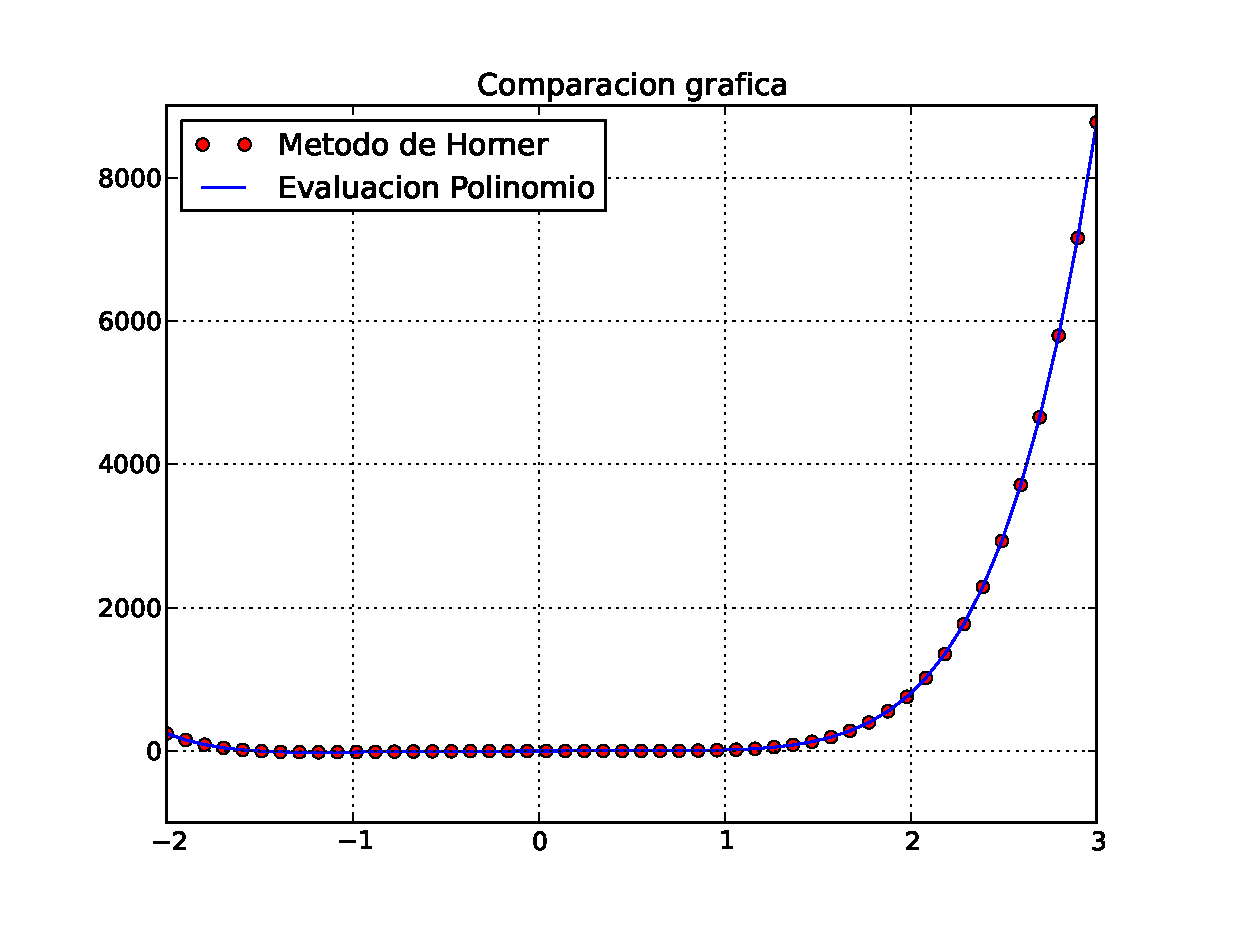
\includegraphics[scale=0.35]{MetodoHorner.eps} 
\end{figure}
\end{frame}
\subsection{El código con \python}
\begin{frame}[fragile]
\frametitle{Estructuramos el código en \python.}
Definimos mediante dos listas:
\setbeamercolor{item projected}{bg=blue!70!black,fg=yellow}
\setbeamertemplate{enumerate items}[circle]
\begin{enumerate}[<+->]
\item Los valores donde queremos evaluar el polinomio $P(x)$.
\item Los coeficientes de $P(x)$.
\end{enumerate}
\begin{lstlisting}[style= FormattedNumber, basicstyle=\linespread{0.9}\ttfamily\normalsize, columns=fullflexible]
# Valores de x0 para evaluar P(x0)
x0=[-1.5, -0.65, 0.1, 1.4, 2.87]

# Coeficientes a de P(x)
a=[2,4,-5,2,-6,8,10]
\end{lstlisting}
\end{frame}
\begin{frame}[fragile]
\frametitle{Definimos una función que resuelva por Horner.}
\fontsize{14}{14}\selectfont
\begin{lstlisting}[style= FormattedNumber, basicstyle=\linespread{0.9}\ttfamily\normalsize, columns=fullflexible]
# Metodo de Horner

def P_Horner(x):
    P_Hor=0
    for n in range(len(a)-1,-1,-1):     
        P_Hor=a[n]+P_Hor*x
    return P_Hor
\end{lstlisting}
\end{frame}
\begin{frame}[fragile]
\frametitle{Definimos una función que evalúe directamente $P(x)$.}
\fontsize{14}{14}\selectfont
\begin{lstlisting}[style= FormattedNumber, basicstyle=\linespread{0.9}\ttfamily\normalsize, columns=fullflexible]
# Evaluacion directa

def P_Directo(x):
    return 2+4*x-5*x**2+2*x**3-6*x**4+8*x**5+10*x**6
    
\end{lstlisting}
\end{frame}
\begin{frame}[fragile]
\frametitle{Calculamos el error relativo.}
\fontsize{14}{14}\selectfont
\begin{lstlisting}[style= FormattedNumber, basicstyle=\linespread{0.9}\ttfamily\normalsize, columns=fullflexible]
# Calculo de error relativo

def Err_Rel(p,p_): return (p-p_)/p*100
\end{lstlisting}
\end{frame}
\begin{frame}[fragile]
\frametitle{Mostramos el error relativo de los puntos a evaluar.}
\fontsize{14}{14}\selectfont
\begin{lstlisting}[style= FormattedNumber, basicstyle=\linespread{0.9}\ttfamily\normalsize, columns=fullflexible]
# Evaluacion de valores de P(x0)

for i in range(len(x0)):                 
    print ("P(%.2f) =" %x0[i],P_Horner(x0[i]), "; Error rel. =", Err_Rel(P_Directo(x0[i]),P_Horner(x0[i])))
\end{lstlisting}
\end{frame}
\begin{frame}[fragile]
\frametitle{Comparamos los resultados con una gráfica.}
\fontsize{14}{14}\selectfont
\begin{lstlisting}[style= FormattedNumber, basicstyle=\linespread{0.9}\ttfamily\small, columns=fullflexible]
import matplotlib.pyplot as plt
import numpy as np

x=np.linspace(-2.,3.)

plt.plot(x,P_Horner(x),'ro', label='Metodo de Horner')

plt.plot(x,P_Directo(x), label='Evaluacion Polinomio')

plt.title('Comparacion grafica')
plt.legend(loc='upper left')

plt.grid(True)
plt.show()
\end{lstlisting}
\end{frame}
\end{document}